\documentclass[a4paper, 14pt]{extreport}

\usepackage[utf8]{inputenc}

\usepackage{icomma}
\usepackage{tabularx}
\usepackage{gensymb}
\usepackage{enumitem}

% % % Page
%\usepackage{extsizes}
\usepackage{geometry}
\geometry{top=20mm}
\geometry{bottom=20mm}
\geometry{left=25mm}
\geometry{right=15mm}

% % % Hyperlinks
\usepackage{hyperref}

% % % Font
\usepackage[T1]{fontenc}
\usepackage[utf8]{inputenc}
\usepackage{mathptmx}
\usepackage{courier}

% % % Pictures
\usepackage{graphicx}

% % % Paragraph
\usepackage{indentfirst}
\linespread{1.3} % 1.5 linespacing

% % % Title
\title{MyPaint\\
\vspace{2mm}
{\large Very simple painting program}}
\author{Oleksandr Redko}
\date{\today}


\begin{document}
	
	\maketitle
	\setcounter{page}{2}
	
	\noindent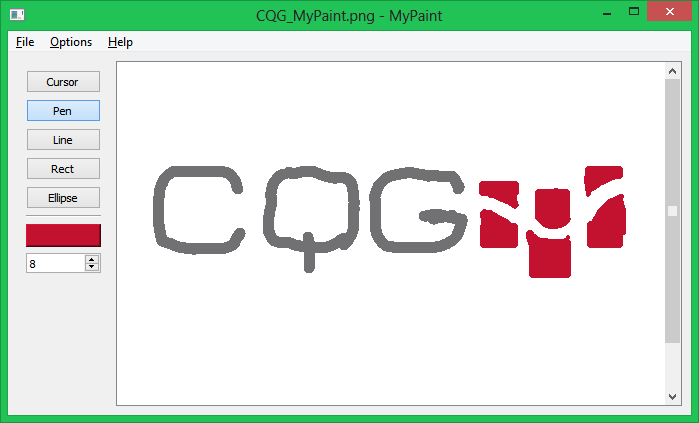
\includegraphics[width=\textwidth]{../CQG_MyPaint_window.png}
	
	With the \textsf{MyPaint} application the users can draw an image.
	There are few instruments for drawing: pencil, tools for painting line, rectangle and ellipse.
	Pen color and width are configurable.
	The \textsf{File} menu gives the users the possibility to open and edit an existing image file, save an image and exit the application.
	\textsf{Options} menu allows users to clear the screen.
	\textsf{Help} menu provides the users with information about the \textsf{MyPaint}.
	
	The program consists of those classes:
	\begin{itemize}
		\item \texttt{PaintScene} inherits \texttt{QGraphicsScene} and allows user to draw on it.
		\item \texttt{InstrumentsWidget} custom Widget that displays control elements for drawing.
		\item \texttt{DataSingleton} is sigleton for store variables and settings of program.
		\item \texttt{AbstractInstrument} is abstract instrument class.
		\item \texttt{PencilInstrument} inherits from \texttt{AbstractInstrument}. 
		\item \texttt{GeometricShapesInstrument} inherits from \texttt{AbstractInstrument}. Draws line, rectangle and ellipse.
		\item \texttt{MainWindow} provides a menu.\textbf{}
	\end{itemize}
	
\end{document}}